\documentclass[a4paper]{article}
\usepackage[utf8]{inputenc}
\usepackage[dvipsnames]{xcolor}
\usepackage[hidelinks]{hyperref}
\usepackage{graphicx, amssymb, amsfonts, color, todonotes, diagbox, colortbl, pdfpages, listings, amsmath, caption, subcaption, xspace, xcolor, pifont, fullpage, algorithm, algpseudocode}
\algnewcommand\algorithmicforeach{\textbf{for each}}
\algdef{S}[FOR]{ForEach}[1]{\algorithmicforeach\ #1\ \algorithmicdo}
\setlength{\parskip}{0.2 cm}
\newtheorem{definition}{Definition}
\newtheorem{theorem}{Theorem}

% Commands
\newcommand{\Node}[1]{\ensuremath{\mathrm{Node}_{#1}}\xspace}
\newcommand{\flow}[1]{\ensuremath{\mathit{flow}_{#1}}\xspace}
\newcommand{\inputs}{\ensuremath{\mathcal{F}}\xspace}
\newcommand{\memory}{\ensuremath{\mathcal{M}}\xspace}
\newcommand{\memorymap}{\ensuremath{\mathcal{M}_{map}}\xspace}
\newcommand{\duration}{\mathit{Duration}\xspace}
\newcommand{\bandwidth}{\mathit{BW}\xspace}
\newcommand{\core}{\mathit{Cores}\xspace}
\newcommand{\submissiontime}{\mathit{Subtime}\xspace}
\newcommand{\walltime}{\mathit{Walltime}\xspace}
\newcommand{\completiontime}{\mathit{Completiontime}\xspace}
\newcommand{\start}{\mathit{Starttime}\xspace}
\newcommand{\fileset}{\ensuremath{\mathbb{F}}\xspace}
\newcommand{\jobset}{\ensuremath{\mathbb{J}}\xspace}
\newcommand{\evict}{\ensuremath{\mathcal{V}}\xspace}
\newcommand{\nbloads}{\ensuremath{\mathit{\mathit{Loads}}}\xspace}
\newcommand{\live}{\ensuremath{L}\xspace}
\renewcommand{\algorithmicrequire}{\textbf{Input:}}
\renewcommand{\algorithmicensure}{\textbf{Output:}}

\title{Data Aware Batch Scheduling}
\author{Maxime GONTHIER - Carl NETTELBLAD - Elisabeth LARSSON \\ Samuel THIBAULT - Loris MARCHAL}
\usepackage[backend=bibtex]{biblatex}
\bibliography{ref}

\begin{document}

\maketitle
\tableofcontents
\listoffigures
\newpage

\todo[inline]{Maxime: You can add highlighted comments this way: "\textbackslash todo[inline]\{Text\}".}
\todo{Maxime: Or with: "\textbackslash todo\\\{Text\}".}

\section{Motivation}

When using a HPC cluster, users may submits tens to hundreds jobs using the same multi-GB input file.
Users tend to submit each such run as a separate batch job.
The job will read inputs directly from a shared file system, which can be disastrous if the number of I/O are important.
We can thus ask ourselves, \textbf{how can we minimize the amount of transfers between the shared file system and the nodes ?}

Users can manually group together input files into a single job to reduce the effects from I/O reads.
Ideally, we would like to let the user submit jobs the way they want and schedule efficiently jobs on nodes.
The workers have a way to store files (with a limit on the memory size), as well as a cache page which contains the files/data recently used.
Thus, a way to minimize data transfers is to create a scheduler that \textbf{take into consideration data locality and schedule on the same node jobs sharing inputs}.

Our scheduler would be used to \textbf{distribute the load between the workers but also to have a vision of what the memory of each worker contains in order to re-use as much as possible a file already loaded on a worker's local memory}.

Clusters already use the efficient SLURM scheduler in order to distribute jobs.
\textbf{Thus our goal is to add a scheduler before the SLURM scheduler that would allocate to each job a node.}

\section{Related Work}

\subsection{About SLURM}
SLURM~\cite{SLURM} is a cluster resource management system, flexible, fault-tolerant and highly scalable.
Schedulers are part of the standard configuration. The Backfill algorithm is very widely used~\cite{New_Backfill}.
Backfill is based on the First Come - First Served principle. While the scheduler is running, jobs in the queue are sorted by priority and queueing time~\cite{New_Backfill}.
If there are not enough nodes to start a job, Backfill takes the next job from the queue and sets it for execution if there are enough nodes for this job and 
it does not delay other jobs.
This algorithm allows to increase the density of supercomputer ressources' use by 20\% as well as reducing the average waiting time
for execution~\cite{Maui_Scheduler}.
Thus our starting point can be the Backfill algorithm.
To be precise, we will be using EASY-Backfilling, a scheduler known to be efficient and able to prevent starvation~\cite{easybf}.
\textbf{We will add a data-aware strategy that maximize data reuse while maintaining EASY-Backfill's basic principle.}

\subsection{Improving SLURM and other batch systems}
To deal with communication-intensive jobs on SLURM, a solution is to minimize network contention by allocating nodes on the least
contended switches~\cite{minimize_network_contention}. In our case we have
jobs with one large file transfers that must be done before the computation start, which is different.
Furthermore, we are scheduling further down the topology (i.e nodes and not switches).

In "Explicit Control in a Batch-Aware Distributed File System"~\cite{Explicit_Control_in_a_Batch-Aware_Distributed_File_System},
we are presented with "Batch-Aware Distributed File System", a system designed to orchestrate large, 
I/O-intensive batch workloads on remote computing clusters.
It adds "storage servers" that export access to the disk. And a scheduler that
manage jobs. 
Like us, they use detailed knowledge of workload characteristics.
However, the main idea is not data reuse but to
facilitates the execution of I/O intensive batch
jobs by selecting appropriate storage policies
in regards to I/O scoping (creating a custom environment for each job
for data that will be used a lot by the job, thus not accessing the main disk too
much) and space allocation.


\subsection{About memory-aware scheduling}
Memory-aware scheduling on clusters have been studied in the past.
 
"Algorithmic Modifications to the
Jacobi-Davidson Parallel Eigensolver to Dynamically Balance External CPU and Memory Load"~\cite{loadbalance_and_trashing} tackle both load balancing and memory constraint. For the load balancing, they 
estimate the time needed by the fastest processor to perform the required $m$ jobs. Thus they can equilibrate the load
with this information. In our study we could use a similar strategy by estimating the 
processing time of a job, the length of a file transfer, and the amount of file transfers needed.
To deal with memory constraint the strategy applied in the paper is to check if 
nodes are thrashing data. If yes, it will recede execution of jobs on this node.
The main differences are that they are using dynamic jobs. Also, we would like to 
manage eviction and optimize data reuse during the scheduling phase, instead of
receding execution on nodes.

Some researchers~\cite{Nikolopoulos2003AdaptiveSU}
are focusing on a better utilization of idling memory together with 
thrashing limitation. Our focus will be to control data loads and eviction so the
processing order will naturally limits thrashing.

\subsection{HDFS, a popular distributed file system}
HDFS~\cite{hdfs} or Hadoop Distributed File System is a distributed file system that incorporate memory-aware scheduling.
HDFS is suitable for applications that have large data sets. 
"Moving Computation is Cheaper than Moving Data" is an important idea for HDFS.
It will migrate a computation closer to where the data is located rather than moving the data to where
the application is running.
Here are our main differences with HDFS. Firstly, HDFS is made for commodity hardware, prone
to more errors and breakdown, so to minimize the risk of failure, data are redundant on the nodes.
In our use case, the scheduler will run on professional clusters and the main point is to load as 
little data as possible. Secondly, HDFS is mainly a storage system, with metadata as transactions historic or
block location. Those concept are not relevant in our use case. Thirdly, the scheduling 
can have issues. A paper describe in detail some problems from MapReduce~\cite{issue_with_hdfs}, the
programming language used in HFDS: the static configuration of the memory allocation, the one-task assigned buffers, the
lake of concurrent task running strategy and the I/O negative impact in memory during the shuffling phase.
To resolve these issues, Mammoth~\cite{Mammoth} was created. It optimize memory usage on a node depending on the hardware configuration.
Our approach is different because we are not dealing with MapReduce or memory allocation.
Our approach is upstream. We can only allocate jobs to nodes. Moreover, we would like to maintain
equity among users  while optimizing I/O.
In addition, HDFS is particularly efficient when the input data used are identical over time.
In our case, one user will submit a lot of different jobs using the same data, but between users,
the inputs are not the same. So HDFS would be less efficient.


\section{Problem Modeling}

\subsection{Framework}
We consider the problem of scheduling independent jobs $J$ on $K$ nodes,
denoted by $\Node{1},\ldots, \Node{K}$.
We denote by $\fileset$ the set of input files and $\jobset$ the set of jobs.
We denote by $\inputs(J_i)$ the set of input files required by job $J_i$. $\inputs(J_i)$ can be empty.
Each file has a size in MB noted $\memory(F_i)$.
Each job has a submission time $\submissiontime(J_i)$ and an 
expected duration time $\duration(J_i)$.
Each job request a certain number of cores $\core(J_i)$. 

\todo[inline]{Maxime: Does all nodes have the same number of cores ? $\rightarrow$ No, 
some nodes will be equipped with 16 cores and other 20.}

\todo[inline]{Can we have situation where a job is requesting more cores than some nodes have ? Like 18 for example ? $\rightarrow$
 ?}

Initially, all input files are stored in the main shared file system.
During the processing of a job $J_i$ on $\Node{k}$, all its inputs
$\inputs(J_i)$ must be in the memory of $\Node{k}$. 
We do not consider the data output of jobs.
Each of the $m$ jobs must be processed on some of the $K$ nodes. 
We consider that all jobs are single nodes.

The file sharing system initially contains all of $\fileset$.
Each node is connected to the file sharing system with a limited bandwidth.
Each node has the same bandwidth noted $\bandwidth$.
The bounded bandwidth as well as the sizes of the files are the reasons why
we aim at restricting the amount of data movement.
\todo[inline]{We would have 2 kind of data ? The first one is an heavy file that need to be copied on 
a local disk (the memory of the node). The second one are small data, using the network file system. This second
type of data do not takes space on the memory of the node ?}

\todo[inline]{Here how I can represent memory map in our model: 
"Each of the $K$ nodes is equipped with a memory of limited size $\memory(\Node{i})$ (in MB).
The memory size can be different among all nodes.
There is locality both across one node and connected with one worker thread:
indeed some jobs use memory map. An other job on the same node can read from this without writing himself beforehand. 
So if a job is co-existing with other jobs using the same file, the memory space taken is smaller.
Thus memory map is used in our cluster. 
Thus a part of $\memory(\Node{i})$ can be used as memory mapping.
The size of this sub-part is $\memorymap(\Node{i})$.}
\todo[inline]{Does these two parts of memory overlap like I wrote ?}
\todo[inline]{Can our input files fit in memory map ? Do only jobs with small input data use memory map ?}

We now define more formally the allocation of the jobs to the node and
their schedule.
We denote by $\sigma(k,i)$ the $i^\text{th}$ job
processed on $\Node{k}$ and by $\evict(k,i)$ the set of file to
be evicted from the memory of $\Node{k}$ before the processing
of this $i^\text{th}$ job ($\evict(k,i)$ can be empty if there is enough space to fit the new files).

On $\Node{k}$, the schedule is made of a
succession of $\mathit{nb}_k$ (the number of jobs allocated) steps, each step being composed of the
following stages (in this order):
\begin{enumerate}
\item Eviction of files if the memory is saturated (we can use flags to force a file to stay in memory. In the same way, we can add a "won't use" flag on a file in order to evict it);
\item The input files in $\inputs(J_{\sigma(k,i)})$ that are not yet in memory are loaded in the memory of $\Node{k}$;
\item Job $J_{\sigma(k,i)}$ is processed on $\Node{k}$ during at most $\duration(J_i)$.
\end{enumerate}
It is important to note that the file transfers are done before the computation and can not be overlapped.

We define the \emph{live data} $\live(k,i)$
as the files in memory of $\Node{k}$ during the computation of $J_{\sigma(k,i)}$, which
can be defined recursively:
$$
\live(k,i)=
\begin{cases}
  \inputs(J_{\sigma(k,1)}) & \text{if~}i=1\\
\Big(\live(k,i-1) \backslash \evict(k,i)\Big) \cup \inputs(J_{\sigma(k,i)})
& \text{otherwise}
\end{cases}
$$

%~ Let's denote $\mathit{Makespan}$, the time it took to execute all of $\jobset$ on a set of $K$ nodes.

%~ Our objective is double:
%~ \begin{itemize}
	%~ \item \textbf{Objective 1: Minimize makespan}
		%~ $$
			%~ \textbf{Obj. 1}: \quad \mathit{minimize}~\mathit{Makespan}
		%~ $$
	%~ \item \textbf{Objective 2: Minimize files movement} 
		%~ The second objective is to limit
	    %~ the amount of file movement, that is, to minimize the sum of the sizes of
	    %~ each file loaded from the file sharing system to the memory of the
	    %~ nodes. We consider that files are not modified. With the
	    %~ natural assumption that no input for job $J_{\sigma(k,i)}$ is
	    %~ evicted from $\Node{k}$ right before its processing
	    %~ ($\evict(k,i) \cap \inputs(J_{\sigma(k,i)}) = \emptyset$), the
	    %~ amount of loads $\memory$ on $\Node{k}$ can be computed as follows:
		%~ $$
			%~ \nbloads_k =\sum_i \memory(\inputs\left(J_{\sigma(k,i)}\right) \backslash \live(k,i-1))
		%~ $$
		%~ Then, our objective is simply to minimize the total number of loads:
		%~ $$
			%~ \textbf{Obj. 2}: \quad  \mathit{minimize} \sum_k \nbloads_k
		%~ $$
%~ \end{itemize}

%~ \begin{definition}[Bi-Obj-Batch-Scheduling]
  %~ Given a number $K$ of nodes, $m$ jobs sharing their inputs files
  % according to a bipartite graph $G$, 
  %~ and two bounds $W$ and $C$, is there a
  %~ schedule $\sigma$ % and an eviction policy $\evict$
  %~ such that $\mathit{Makespan} \leq W$ and $\sum_k \nbloads_k \leq C$?
%~ \end{definition}

%~ Load balancing/minimizing makespan and file re-use can be two opposing goals, so we would like to measure the impact on the performance depending on the strategy (Focus on load balancing or focus on file re-use or both for example) ?

\subsection{Formalization of the objective}
\textbf{Objective: Minimize the maximum \flow{}}
		We define the \flow{J_i} of a job as:
		$$
			\flow{J_i} = \completiontime(J_i) - \submissiontime(J_i)
		$$
		Our goal is:
		$$
			\textbf{Obj.}: \quad \mathit{minimize}~\mathit{max}(\flow{J_1}, \flow{J_2}, ..., \flow{J_m})
		$$
	%~ \item \textbf{Objective 2: Minimize files movement} 
		%~ The second objective is to limit
	    %~ the amount of file movement, that is, to minimize the sum of the sizes of
	    %~ each file loaded from the file sharing system to the memory of the
	    %~ nodes. We consider that files are not modified. With the
	    %~ natural assumption that no input for job $J_{\sigma(k,i)}$ is
	    %~ evicted from $\Node{k}$ right before its processing
	    %~ ($\evict(k,i) \cap \inputs(J_{\sigma(k,i)}) = \emptyset$), the
	    %~ amount of loads $\memory$ on $\Node{k}$ can be computed as follows:
		%~ $$
			%~ \nbloads_k =\sum_i \memory(\inputs\left(J_{\sigma(k,i)}\right) \backslash \live(k,i-1))
		%~ $$
		%~ Then, our objective is simply to minimize the total number of loads:
		%~ $$
			%~ \textbf{Obj. 2}: \quad  \mathit{minimize} \sum_k \nbloads_k
		%~ $$
A secondary objective is to minimize the amount of file loaded in MB.
Indeed, loading files has a huge impact on the total makespan and thus on the maximum \flow{}.

\section{Other measurements}

Each job has a start time $\start(J_i)$, the actual time at which the job was executed.
We also want to measure the average queue time of a job in order
to evaluate our scheduler in terms of fairness. We can do:
$$
	Average\_queue\_time = \frac{\sum^{m}_{i = 0} \start(J_i) - \submissiontime(J_i)}{m}
$$

We also want to measure the core-hours used. We need to take into consideration the amount of files loaded before the computation.
With $\core(J_i)$ the number of processor units used by job $i$ and $\duration(J_i)$ the duration of job $i$ in hours, we have:
$$
	\#Corehours = \sum^{m}_{i = 0} \core(J_i) \times (\duration(J_i) + \frac{\memory(\inputs\left(J_{\sigma(k,i)}\right) \backslash \live(k,i-1)))}{\bandwidth}
$$

\section{The use of simulation}

The use of simulation is motivated both by the fidelity of simulated results as well as energy savings. 
We will be using Batsim, a precise and realistic~\cite{Batsim} resource and job management system (RJMS) simulator.
Batsim JSON-formatted workloads are extensible and allow easy workload generation. 
Moreover, Batsim provides clear information about scheduling metrics and job placement.
We will add a scheduler using Batsched~\footnote{\url{https://gitlab.inria.fr/batsim/batsched}}.

\paragraph{Data mining for an accurate simulation}
A number of informations must be retrieved in order to accurately 
simulate the use case of Uppsala's University cluster:
\begin{itemize}
	\item	.xml files of the cluster containing informations on the nodes.
	\item	Bandwidth of each node in order to compute the estimated time of a file load with: $\frac{\memory(F_i)}{\mathit{Bandwidth(\Node{i})}}$.
	\item	Size of input files (20 to 100 GB ?)
	\item	Duration of jobs
	\item	Are some files more popular ?
	\item	Total number of jobs
	\item	Number of available nodes
	\item	Size of node's memory (128 GB ?)
\end{itemize}

\paragraph{How to simulate data transfers ?}
We can add dynamic job of duration the time it would take to transfer the file on the node in order
to simulate file loads.

\section{Algorithm}

When we need to choose a node for job $J_i$ we know the following informations:
\begin{itemize}
	\item $\submissiontime(J_i)$
	\item $\walltime(J_i)$
	\item $\inputs(J_i)$
	\item Size of files for the job: $\memory(\inputs(J_i))$
	\item For each $i$, $\inputs(\Node{i})$
	\item Size of files already on memory of the node: For each $i$, $\memory(\inputs(\Node{i}))$
	\item Bandwidth: $\bandwidth$
	\item Memory that was mapped ?
\end{itemize}

\paragraph{Intuition} 
We could estimate the time it will take to transfer all of the input files of job $J_i$ depending on the node:
$$
	\mathit{Transfertime\_J_i}(\Node{j}) = \frac{\memory(\inputs(J_i) \notin \inputs(\Node{j}))}{\bandwidth}
$$

With this information we can do two things:
\begin{itemize}
	\item Schedule $J_i$ on an available node $j$ that achieve $min(\mathit{Transfertime\_J_i}(\Node{j}))$
	\item Schedule $J_i$ on an non-available node $j$ such as $\mathit{Transfertime\_J_i}(\Node{j}) + \walltime(current~job~on~node~j) < min(\mathit{Transfertime\_J_i}(\Node{k})), k \in available~nodes$
\end{itemize}

\todo[inline]{Maxime: Does it make sense ?}

\begin{algorithm}[htbp]
	\caption{Data Aware Batch Scheduler (DABS)}\label{algo.dabs}
\hspace*{\algorithmicindent} \textbf{Input: job $J_i$, set of node} \\
 %~ \hspace*{\algorithmicindent} \textbf{Output: $\sigma$}
	\begin{algorithmic}[1]
		\State  
		%~ \State For each \GPU{k}, $\mathit{InMem}(k)\gets \emptyset$
		%~ \While{all tasks have not been allocated}
		%~ \State  $T_i\gets \mathit{pop}(\taskset)$
		%~ \State For each \GPU{k}, compute $C_k(T_i)$ using Eq.~\ref{eq.dmda_model}
		%~ \State Select $k$ such that $C_k(T_i)$ is minimal
		  %~ \State Allocate $T_i$ on \GPU{k}
		  %~ \For{each $D_i \in \inputs(T_i)$}
		  %~ \State Request data prefetch for $D_j$ on \GPU{k}
		  %~ \State Add $D_i$ to $\mathit{InMem}(k)$
		  %~ \EndFor
		  %~ \EndWhile
	\end{algorithmic}
\end{algorithm}

\section{Algo}

\subsection{Random-Available-Job-on-Random-Node (RAJ-RN)}
Schedule a random available job on a random node even if it's not available, it will be schedule for later execution on this node.

\subsection{Random-Available-Job-on-Random-Available-Node (RAJ-RAN)}
Schedule a random available job on a random available node.

\subsection{First-Come-First-Serve (FCFS)}
Schedule the job submitted the earliest on the first available node from the node list (So node 1 if it is available, else node 2 and so on...)

\subsection{First-Come-First-Serve-Data-Aware (FCFS-DA)}
Schedule the job submitted the earliest on the available node from the node list with which it shares the most data. If there is a tie we choose the node with the smallest index.

\section{Experiments}

% Queue times
\begin{figure}[ht] 
  \label{ fig7} 
  \begin{minipage}[b]{0.5\linewidth}
    \centering
    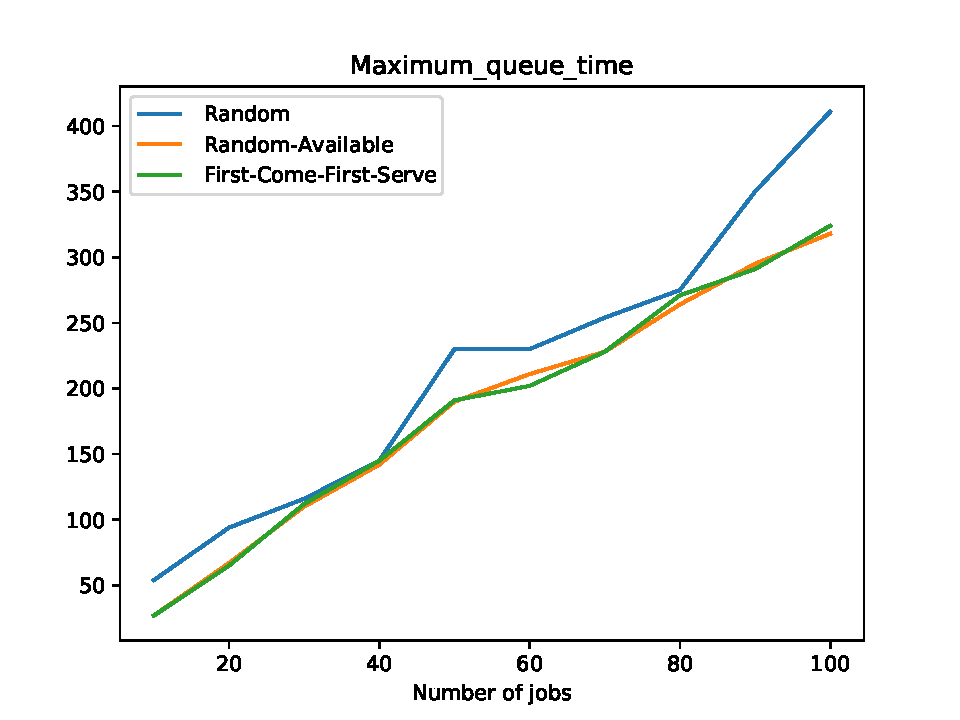
\includegraphics[width=1.11\linewidth]{MBSS/plot/Maximum_queue_time.pdf} 
    \caption{maximum queue time} 
    \vspace{4ex}
  \end{minipage}%%
  \begin{minipage}[b]{0.5\linewidth}
    \centering
    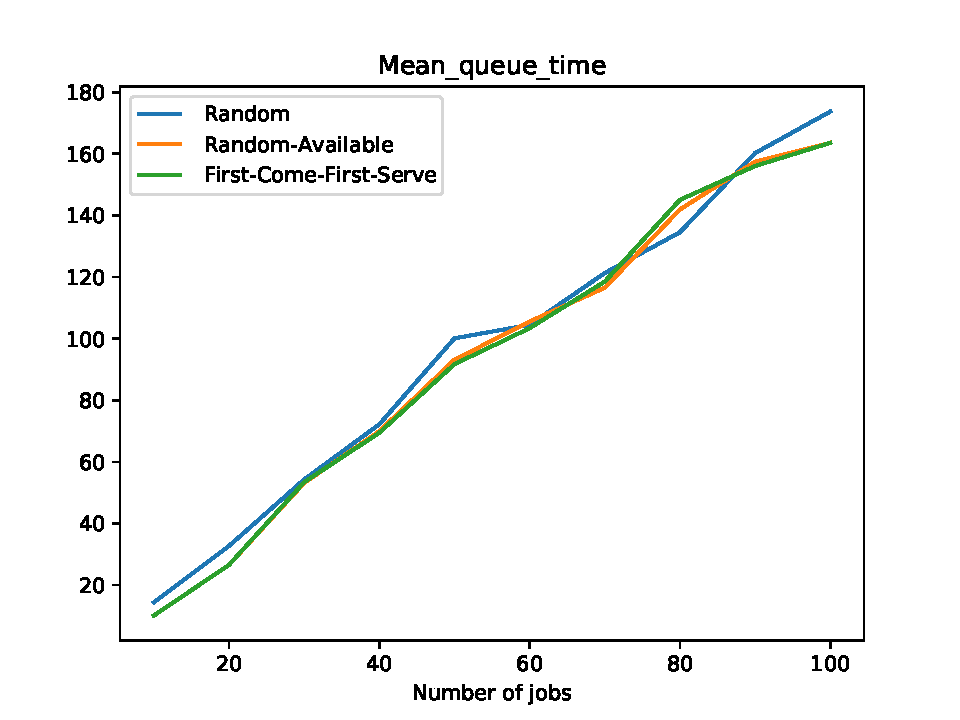
\includegraphics[width=1.11\linewidth]{MBSS/plot/Mean_queue_time.pdf} 
    \caption{Mean queue time} 
    \vspace{4ex}
  \end{minipage} 
  \begin{minipage}[b]{0.5\linewidth}
    \centering
    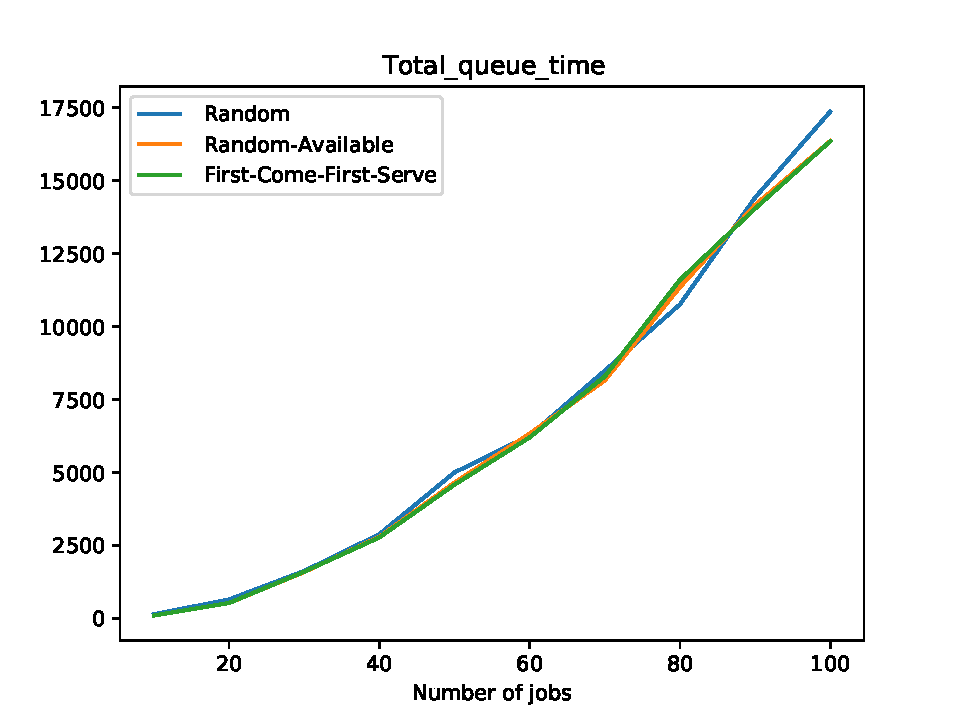
\includegraphics[width=1.11\linewidth]{MBSS/plot/Total_queue_time.pdf} 
    \caption{Total queue time} 
    \vspace{4ex}
  \end{minipage}%% 
  \begin{minipage}[b]{0.5\linewidth}
    \centering
    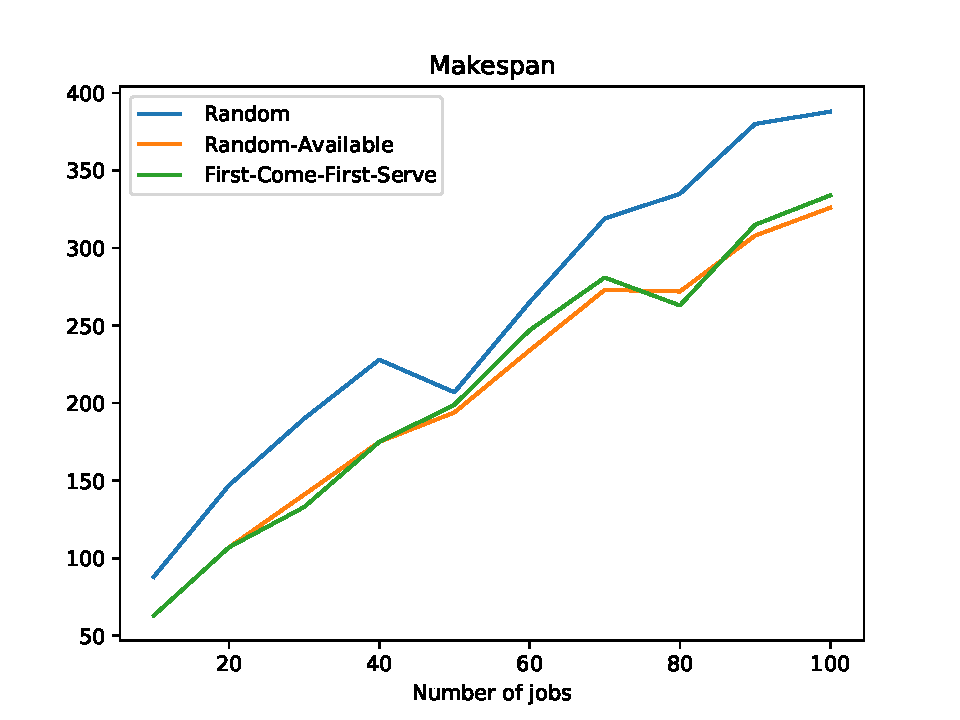
\includegraphics[width=1.11\linewidth]{MBSS/plot/Makespan.pdf} 
    \caption{Makespan} 
    \vspace{4ex}
  \end{minipage} 
\end{figure}

% Flow
\begin{figure}[ht] 
  \label{ fig7} 
  \begin{minipage}[b]{0.5\linewidth}
    \centering
    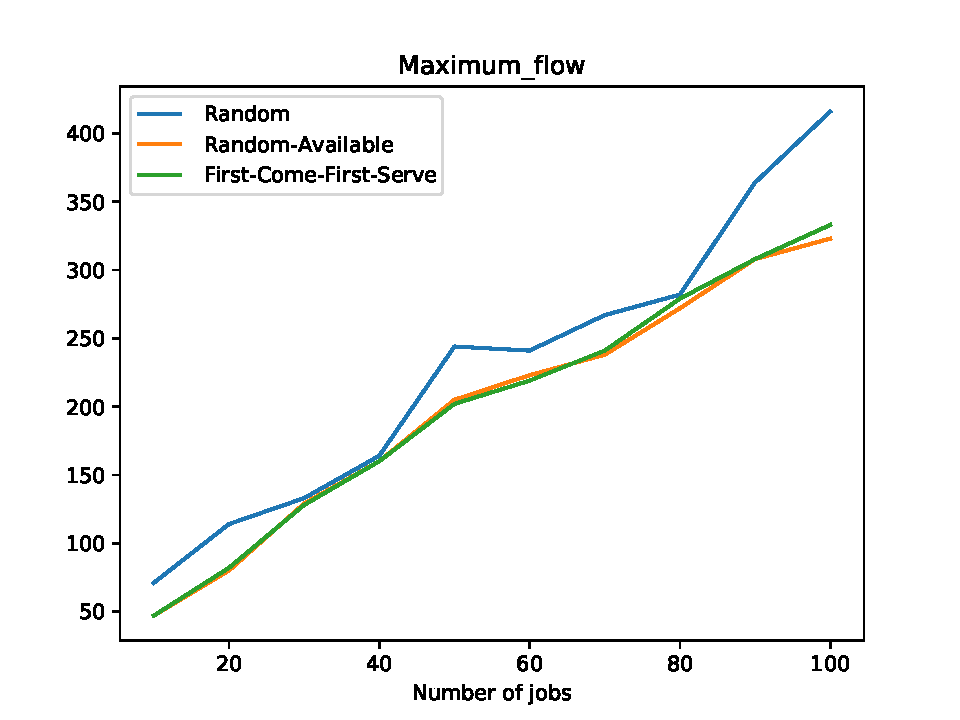
\includegraphics[width=1.11\linewidth]{MBSS/plot/Maximum_flow.pdf} 
    \caption{Maximum flow} 
    \vspace{4ex}
  \end{minipage}%%
  \begin{minipage}[b]{0.5\linewidth}
    \centering
    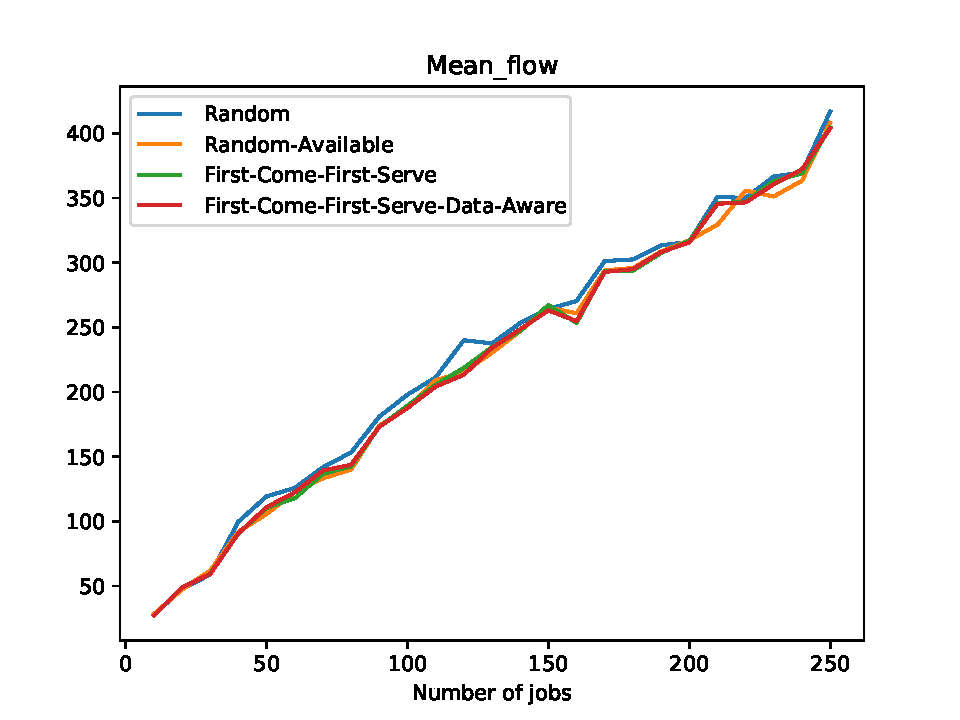
\includegraphics[width=1.11\linewidth]{MBSS/plot/Mean_flow.pdf} 
    \caption{Mean flow} 
    \vspace{4ex}
  \end{minipage} 
  \begin{minipage}[b]{0.5\linewidth}
    \centering
    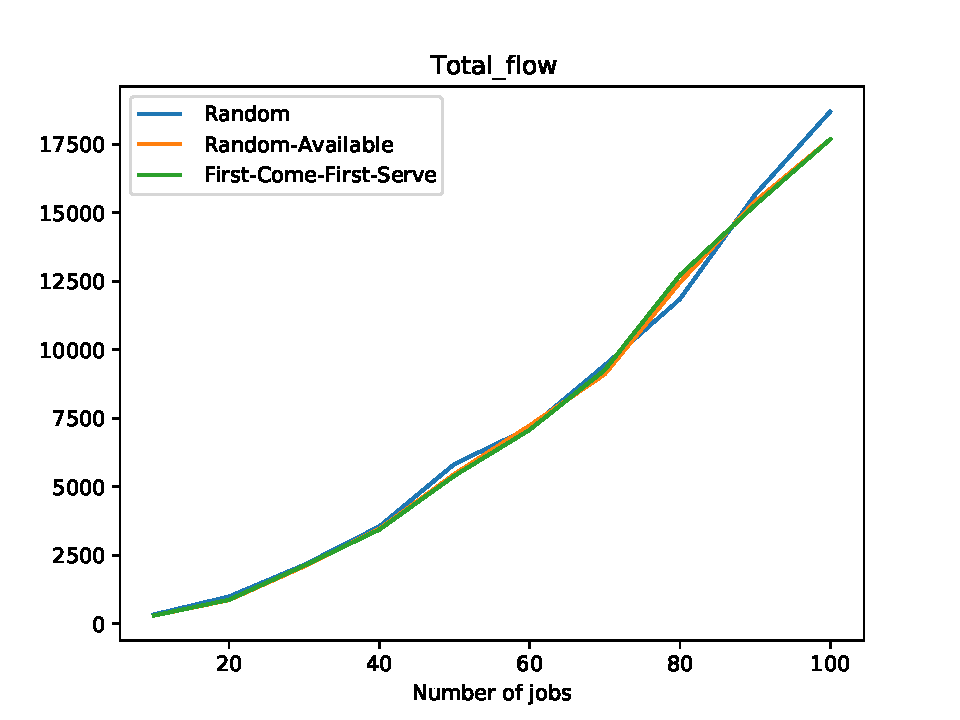
\includegraphics[width=1.11\linewidth]{MBSS/plot/Total_flow.pdf} 
    \caption{Total flow} 
    \vspace{4ex}
  \end{minipage}%% 
  \begin{minipage}[b]{0.5\linewidth}
    \centering
    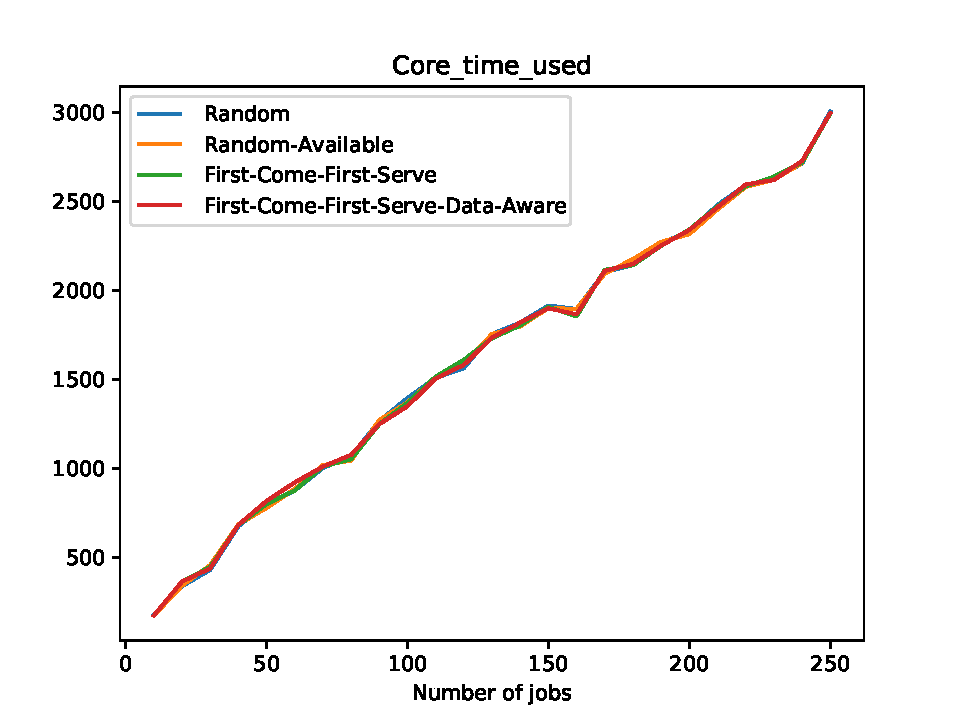
\includegraphics[width=1.11\linewidth]{MBSS/plot/Core_time_used.pdf} 
    \caption{Core time used} 
    \vspace{4ex}
  \end{minipage} 
\end{figure}

% Transfer time
\begin{figure}[ht]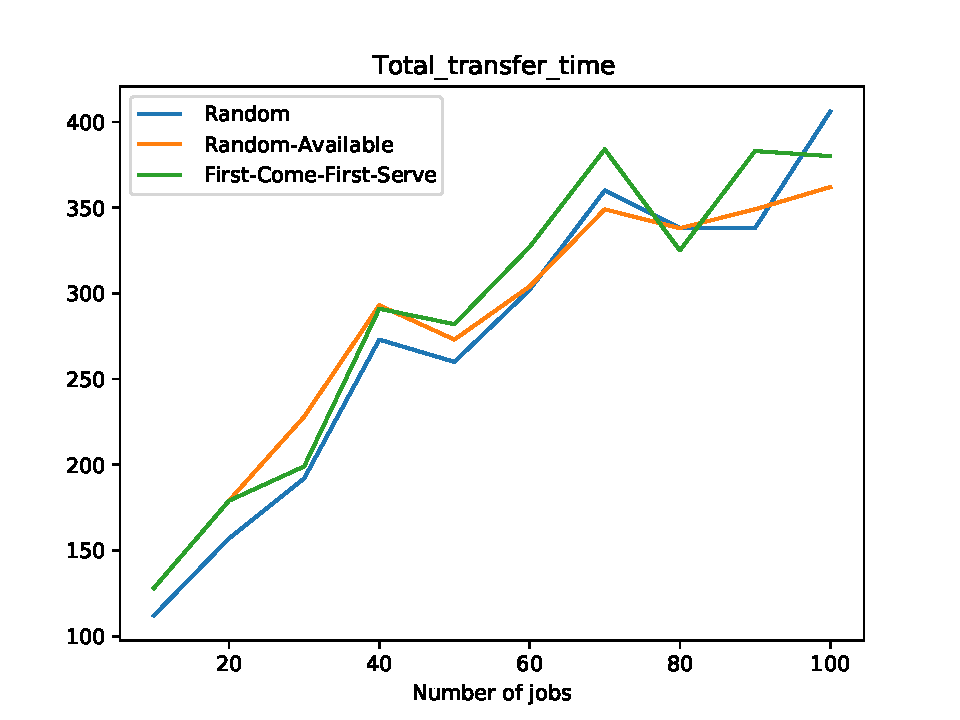
\includegraphics[scale=1]{MBSS/plot/Total_transfer_time.pdf}\caption{Transfer time}\end{figure}

% gantt charts
\begin{figure}[ht] 
  \label{ fig7} 
  \begin{minipage}[b]{0.5\linewidth}
    \centering
    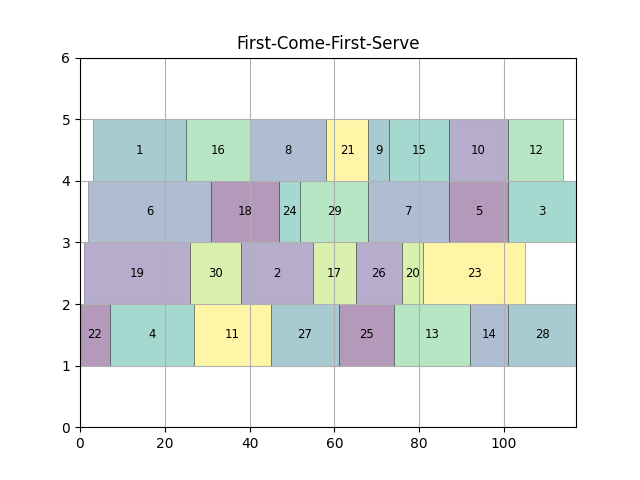
\includegraphics[width=1.11\linewidth]{MBSS/plot/Gantt_charts/First-Come-First-Serve.png} 
    \caption{} 
    \vspace{4ex}
  \end{minipage}%%
  \begin{minipage}[b]{0.5\linewidth}
    \centering
    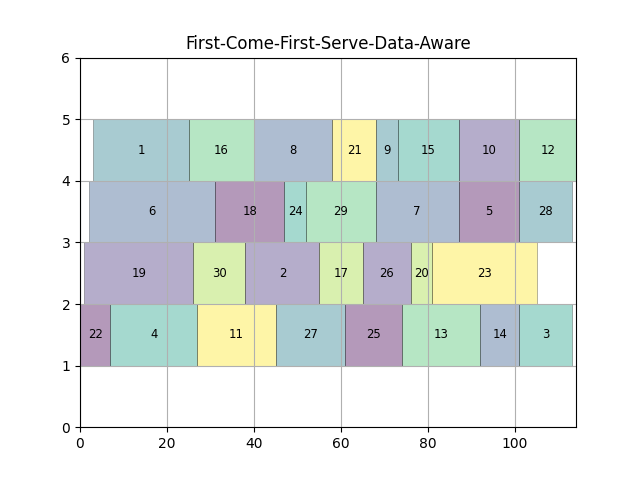
\includegraphics[width=1.11\linewidth]{MBSS/plot/Gantt_charts/First-Come-First-Serve-Data-Aware.png} 
    \caption{} 
    \vspace{4ex}
  \end{minipage} 
  \begin{minipage}[b]{0.5\linewidth}
    \centering
    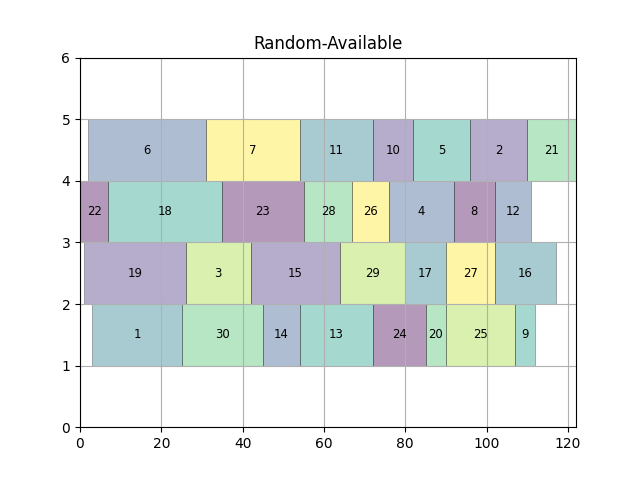
\includegraphics[width=1.11\linewidth]{MBSS/plot/Gantt_charts/Random-Available.png} 
    \caption{} 
    \vspace{4ex}
  \end{minipage}%% 
\end{figure}

\printbibliography
\end{document}
